\documentclass{beamer}

\usepackage[utf8]{inputenc}
\usepackage{graphicx}
\usepackage{multimedia}
\usepackage{url}

\usetheme{default}
\usecolortheme{crane}
\usefonttheme{default}
\useoutertheme{sidebar}
\useinnertheme[shadow=true]{rounded}

\title{Jeu du Pérudo}
\author{H4104 - Dragibus}
\institute{INSA de Lyon}
\logo{
\includegraphics[height=8mm, width=14mm]{logo.jpg}}

\begin{document}

\begin{frame}
  \titlepage
\end{frame}

\begin{frame}
  \frametitle{Sommaire}
  \tableofcontents[hideallsubsections]
\end{frame}

\section{Mécanisme du jeu}

\begin{frame}
  \frametitle{Principe}

  \begin{figure}
    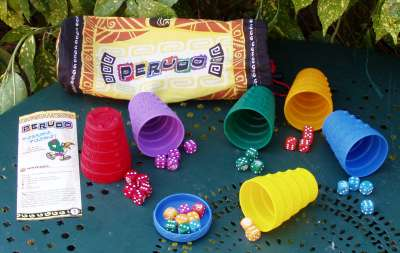
\includegraphics[scale=0.4]{perudo.jpg}
  \end{figure}

  \begin{itemize}
    \item jeu de dés
    \item multijoueur, entre 2 et 6 (ou plus) joueurs
    \item deviner le nombre de dés d'une valeur, connaissant seulement ses
      propres dés
    \item dernier joueur ayant des dés gagne la partie
  \end{itemize}
\end{frame}

\begin{frame}
  \frametitle{Règles}
  $\to$ parier sur le nombre de dés en jeu \\
  \emph{(pour une certaine valeur de dé)}

  \begin{itemize}
    \item dudo : "douter", soit réfuter la mise actuelle
    \item calza : "calé", affirmer que la mise actuelle est exacte
    \item enchêre : augmenter le nombre de dés ou changer la valeur du dé
  \end{itemize}

  \uncover<2-3>{
    \textbf{Exemple}
    \\
    Joueur précédent : \textit{"Je pense qu'il y a douze 5"}
    \\
    Moi :\textit{"Je pense qu'il y a treize 5"}
  }
  \\[5mm]
  \uncover<3>{
    $\to$ la mise ne peut qu'\textbf{augmenter} au cours de la partie
  }
\end{frame}

\section{Concept d'IA}

\begin{frame}
  \frametitle{Constat}

  À son tour, le joueur doit \textbf{évaluer} les différents coups possibles.
  \\[1.5cm]
  \begin{center}
    \uncover<2>{\textit{Une IA devrait fonctionner de la même manière.}}
  \end{center}
\end{frame}

\begin{frame}
  \frametitle{Évaluation}

  \begin{itemize}
    \item état de soi-même (dés)
    \item état du jeu (mise précédente, historique des mises, nombre de dés)
    \item coups possibles
  \end{itemize}

  \center{$ia(EtatJoueur, EtatJeu, CoupsPossibles) \to Evaluation$}
  \\[1cm]
  \large L'IA est une \textbf{fonction d'évaluation} de l'état du jeu.
\end{frame}

\begin{frame}
  \frametitle{Combinaison}

  \begin{large}
    Permet de créer des IA complèxes à partir d'autres relativement simples.
    \\[1cm]
    \uncover<2>{Combinaison linéaire avec des coefficients de
      \emph{poids}, correspondant à la prise en compte dans la décision
      finale.}
  \end{large}
\end{frame}

\section{Présentation des IA}

\begin{frame}
  \frametitle{Basiques}

  \textbf{Stochastique}
  \\
  Fonctionnement : associe à chaque coup une estimation aléatoire.
  \\
  Résultat attendu : inattendu.
  \\[1cm]
  \textbf{Minimale}
  \\
  Fonctionnement : joue à son tour le coup le moins risqué.
  \\
  Résultat attendu : taux de victoire stable et moyen.
\end{frame}

\begin{frame}
  \frametitle{Probabiliste}

  Fonctionnement : associe à chaque coup la probabilité qu'il soit présent.

  Pour un nombre de dés $n$ "inconnus", la probabilité $P(q)$ qu'il y ait
  \emph{au moins} la quantité $q$ de la valeur souhaitée est de :

  $$
  \sum\limits_{x=q}^n C(n, x) \cdot (1/6)^x \cdot (5/6)^{n-x}
  $$

  Où C(n, q) est le coefficient binomial (q parmi n).
  \\[1cm]

  Résultat attendu : taux de victoire stable et élevé.
\end{frame}

\begin{frame}
  \frametitle{Apprentissage}

  Fonctionnement : associe à chaque joueur un indice de confiance maintenu au
  cours de la partie. Correspond au taux de "bluff" du joueur, calculé à chaque
  fin de tour par la distance entre les mises du joueur et son jeu réel. L'IA
  considèrera que si un joueur a une confiance de $C$ et a misé une mise de
  $Nb$ dés il y a en réalité $C \cdot Nb$ dés, et prendra la valeur maximale
  pour tous les joueurs.
  \\[1cm]
  Résultat attendu : croissance du taux de victoire au cours du temps.
\end{frame}

\section{Résultats et observations}

\end{document}

% vim: et sw=2 sts=2
